% !TEX root = ../dg.tex

\section{Integral Curves and Lie Derivatives}

To motivate the definition of the Lie bracket, I claimed that there was additional algebraic structure on $\mathfrak{X}(M)$ in the form of a binary operation, and then (hopefully!) convinced you that there was really only one sensible way to define such an operation.

But it's probably not at all obvious why one should have guessed that there was a binary operation on vector fields in the first place, and, though I don't actually know the history, my guess is that this was not the original motivation for the Lie bracket.

In some sense the more basic notion is that of the \emph{Lie derivative}, which is a sort of directional derivative of vector fields which, as we will see, actually generalizes to arbitrary tensor fields.

The idea is that, given two vector fields $X$ and $Y$ on a manifold $M$, we might like to define a ``directional derivative of $Y$ in the direction of $X$'' operator, which we will denote $\mathcal{L}_XY$, where the $\mathcal{L}$ is for ``Lie derivative.'' It will turn out that $\mathcal{L}_XY = [X,Y]$, which might be surprising, but if you look back to the local coordinate expression~\eqref{eq:Lie bracket in local coords} for $[X,Y]$, you'll notice it involved differentiating the coefficients of $Y$ with respect to $X$ (and also $X$ with respect to $Y$, but we'll shortly see why there's this symmetry).

It's worth thinking for yourself about how you might go about defining such a derivative operator, so I would encourage you to do so before reading on.

Here's a way of making this ``directional derivative for vector fields'' operation more precise: say we have our vector fields $X$ and $Y$ and we want to compute $\mathcal{L}_XY$ at a point $p \in M$. Presumably the idea is to measure how much $Y$ is changing as we vary $p$ in the direction of $X$. 

In other words, we want to integrate $X$ to get a curve $\alpha: (-\epsilon, \epsilon) \to M$ so that $\alpha(0) = p$ and $\alpha'(t) = X(\alpha(t))$ for all $t \in (-\epsilon, \epsilon)$, then look at something like
\[
	\lim_{t\to 0} \frac{Y(\alpha(t))-Y(\alpha(0))}{t}.
\]
See \cref{fig:lie-derivative}.

\begin{figure}[htbp]
	\centering
		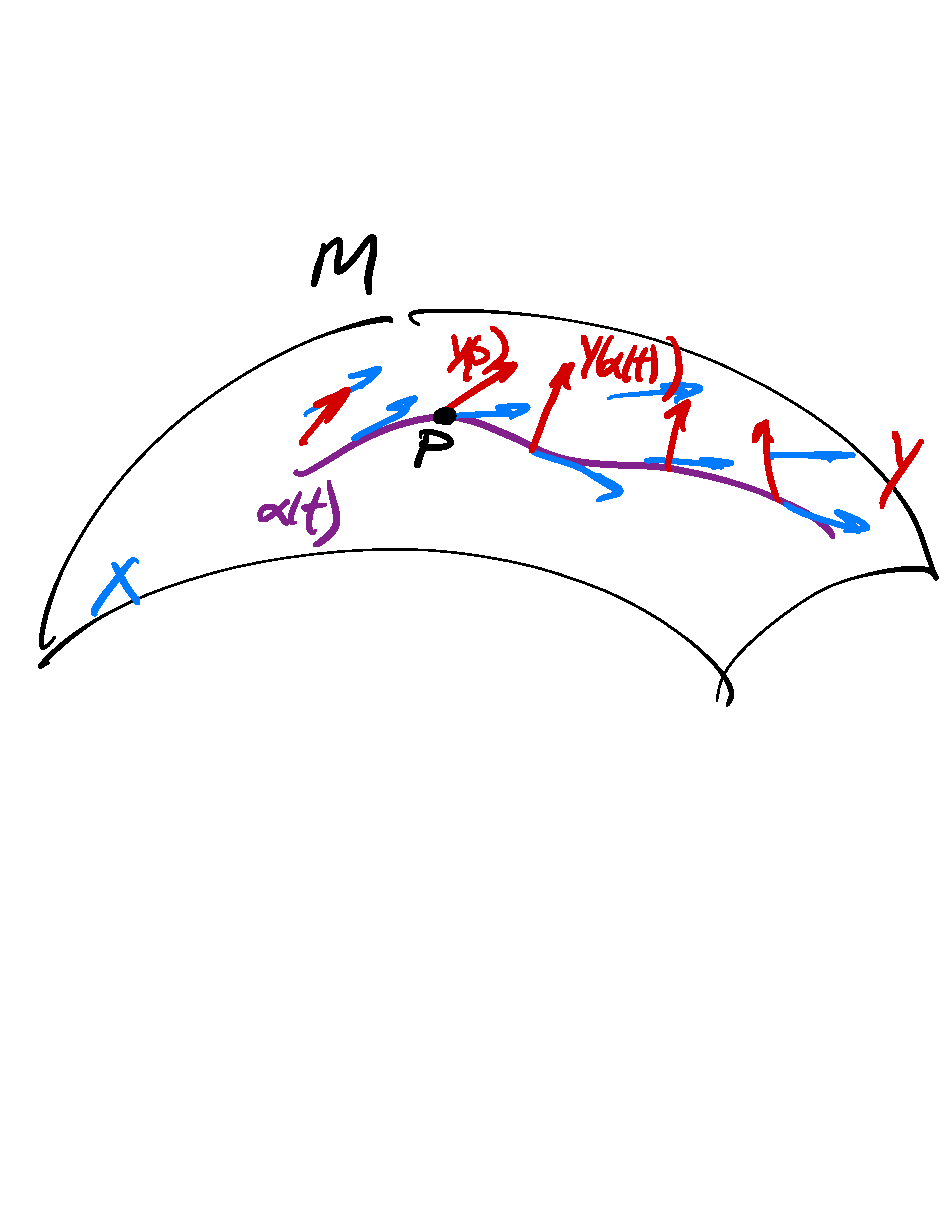
\includegraphics[height=1.5in]{lie-derivative}
	\caption{An attempt to differentiate $Y$ in the direction of $X$.}
	\label{fig:lie-derivative}
\end{figure}

In other words, we look at the rate of change of $Y$ as we flow in the direction of $X$. Unfortunately, as written the above difference quotient doesn't make sense, but first let's talk about flows and integrating vector fields.

\begin{definition}\label{def:integral curve}
	Let $X \in \mathfrak{X}(M)$. A curve $\alpha\from (a,b) \to M$ is called an \emph{integral curve} (or \emph{trajectory}) for $X$ if $\alpha'(t) = X(\alpha(t))$ for all $t \in (a,b)$. 
\end{definition}

\begin{proposition}\label{prop:local flow}
	Let $X \in \mathfrak{X}(M)$ and let $p \in M$. Then there exists a neighborhood $U$ of $p$, a $\delta > 0$, and a smooth map $\Phi\from (-\delta, \delta) \times U \to M$ so that, for each $q \in U$, the map $t \mapsto \Phi(t,q)$ is the unique smooth curve satisfying the ODE $\frac{\partial \Phi}{\partial t} = X(\Phi(t,q))$ with initial condition $\Phi(0,q) = q$. See \cref{fig:local-flow}.
\end{proposition}

\begin{figure}[htbp]
	\centering
		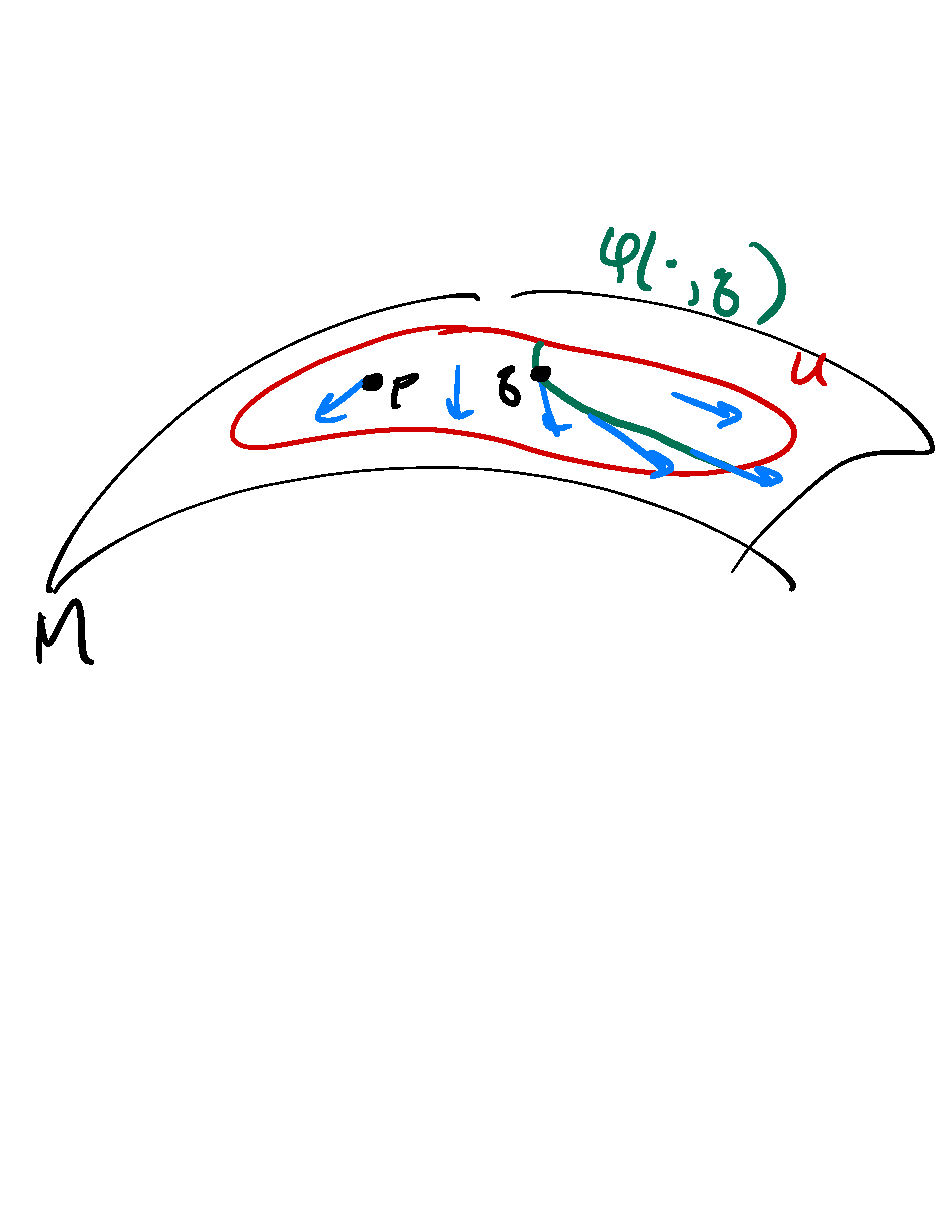
\includegraphics[height=1.5in]{local-flow}
	\caption{The local flow generates an integral curve through each point.}
	\label{fig:local-flow}
\end{figure}

\begin{proof}
	Since $M$ is locally diffeomorphic to $\R^n$ (via the coordinate charts), this follows from the fundamental theorem on existence and uniqueness of solutions to ODEs in $\R^n$.
\end{proof}

We often use the notation $\Phi_t(q):=\Phi(t,q)$ and call $\Phi_t$ the \emph{local flow} of $X$.

\begin{example} 
	Let $M = S^2$ and consider the vector field $X(x,y,z) = zx \frac{\partial}{\partial x} + zy \frac{\partial}{\partial y} +\left(z^2-1\right) \frac{\partial}{\partial z}$ (of course, this is written in extrinsic $\R^3$ coordinates rather than intrinsic coordinates). See \cref{fig:flowfield}.
	
	\begin{figure}[htbp]
		\centering
			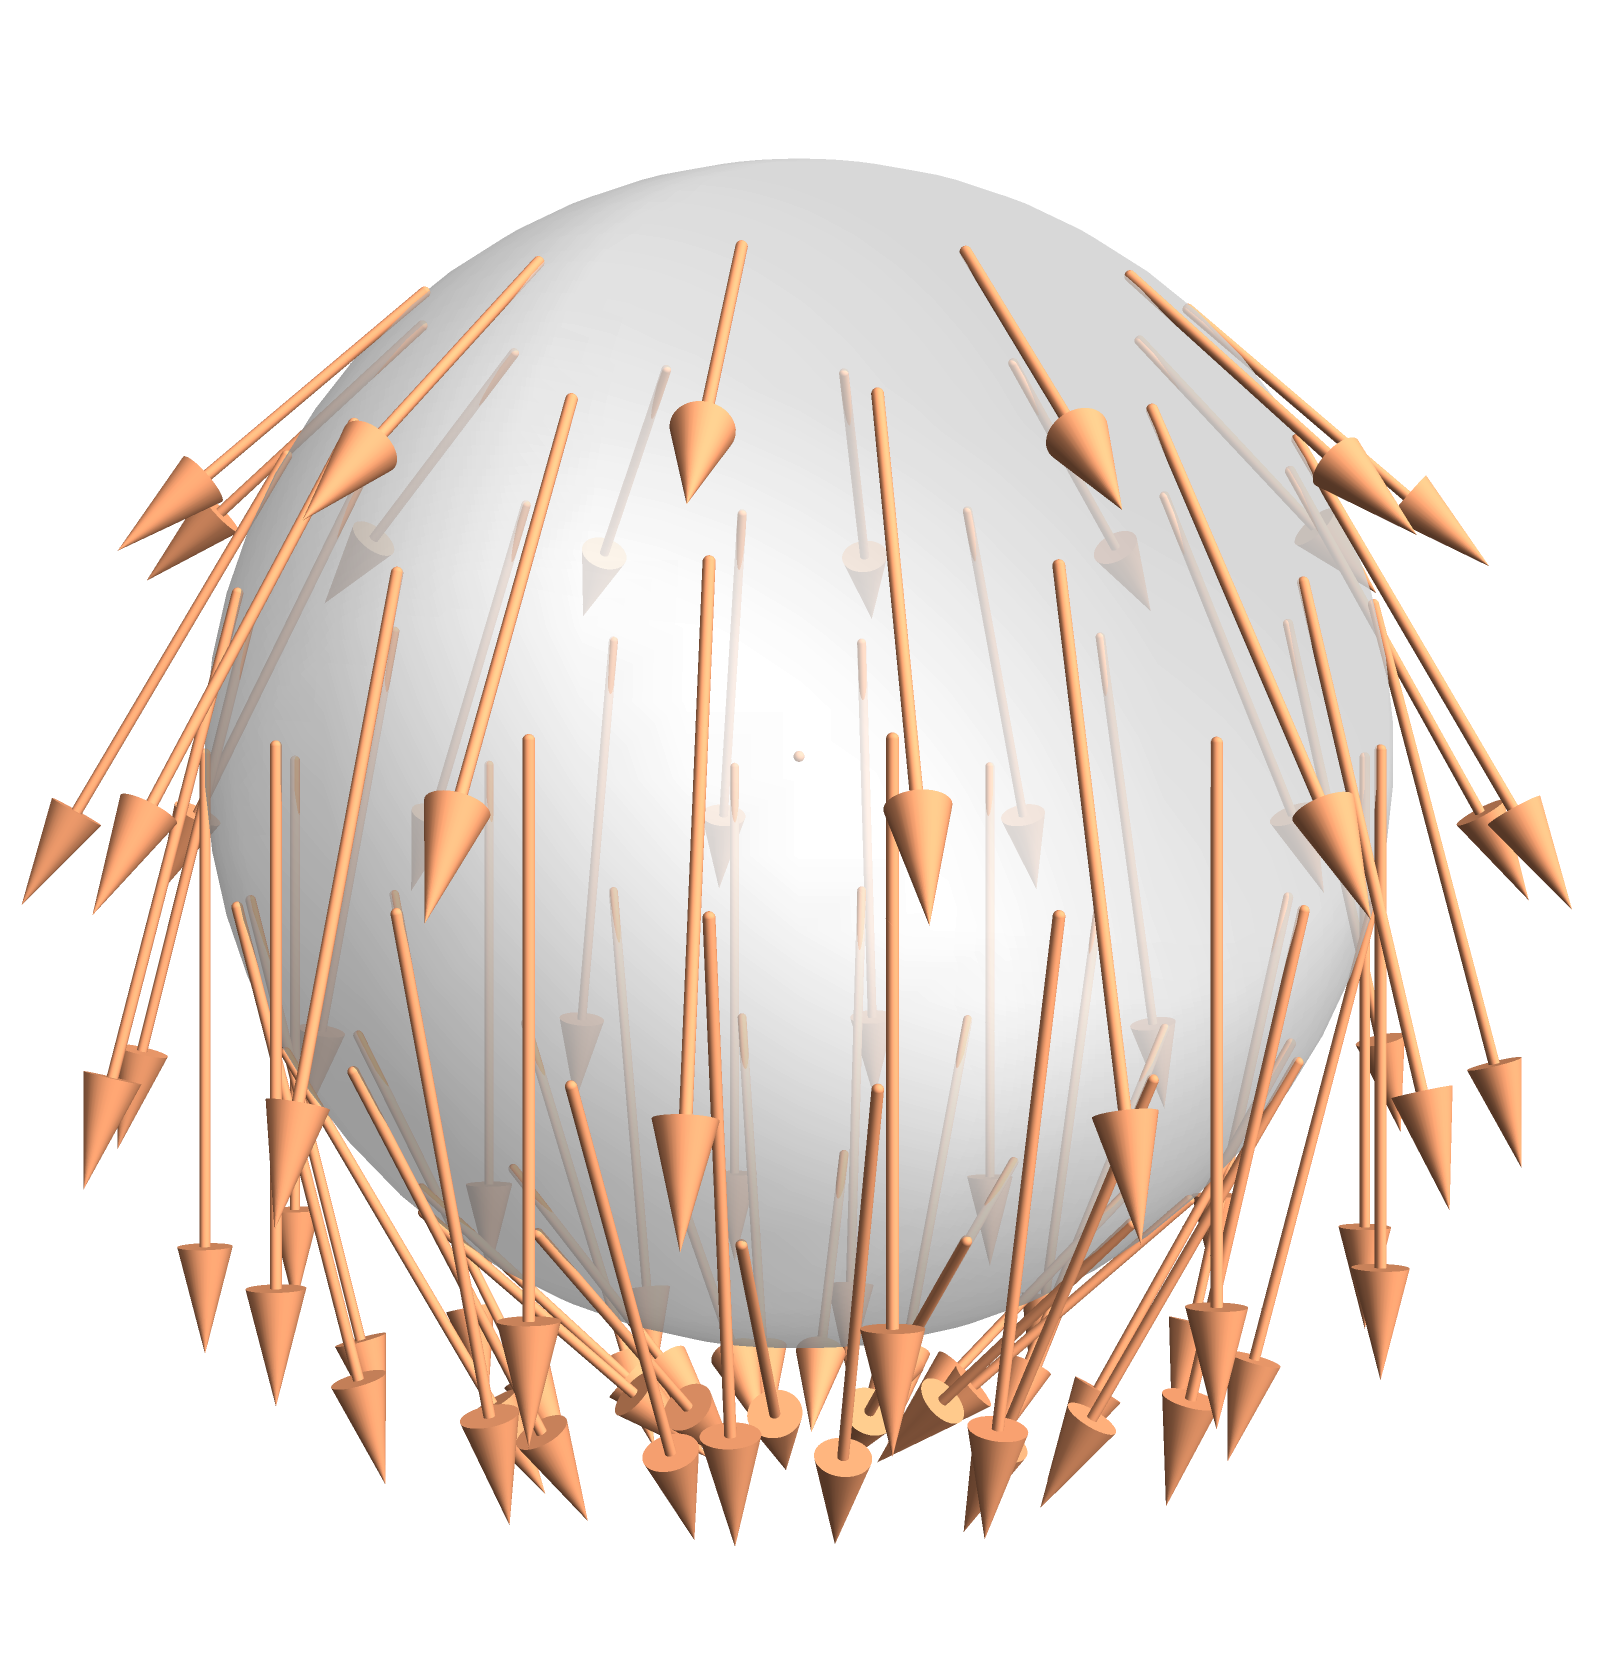
\includegraphics[height=2in]{flowfield}
		\caption{The vector field $X(x,y,z) = zx \frac{\partial}{\partial x} + zy \frac{\partial}{\partial y} +\left(z^2-1\right) \frac{\partial}{\partial z}$ on the sphere.}
		\label{fig:flowfield}
	\end{figure}
	
	In fact, you can check that this is just $(d\phi_N)Y$, where $Y$ is the vector field on $\R^2$ given by $Y(u,v) = -u \frac{\partial}{\partial u} - v \frac{\partial }{\partial v}$.
	
	Visually, the local flow pushes the mass of the sphere down towards the south pole. We can integrate the flow explicitly in \emph{Mathematica} to get
	\[
		\Phi_t(x,y,z) = \frac{1}{1+2e^{2t} + \left(1-e^{2t}\right)z}\left(2e^t x, 2e^t y, 1-e^{2t} + \left(1+e^{2t}\right)z\right).
	\]
	See \cref{fig:conformalflow}.
	
	\begin{figure}[htbp]
		\centering
			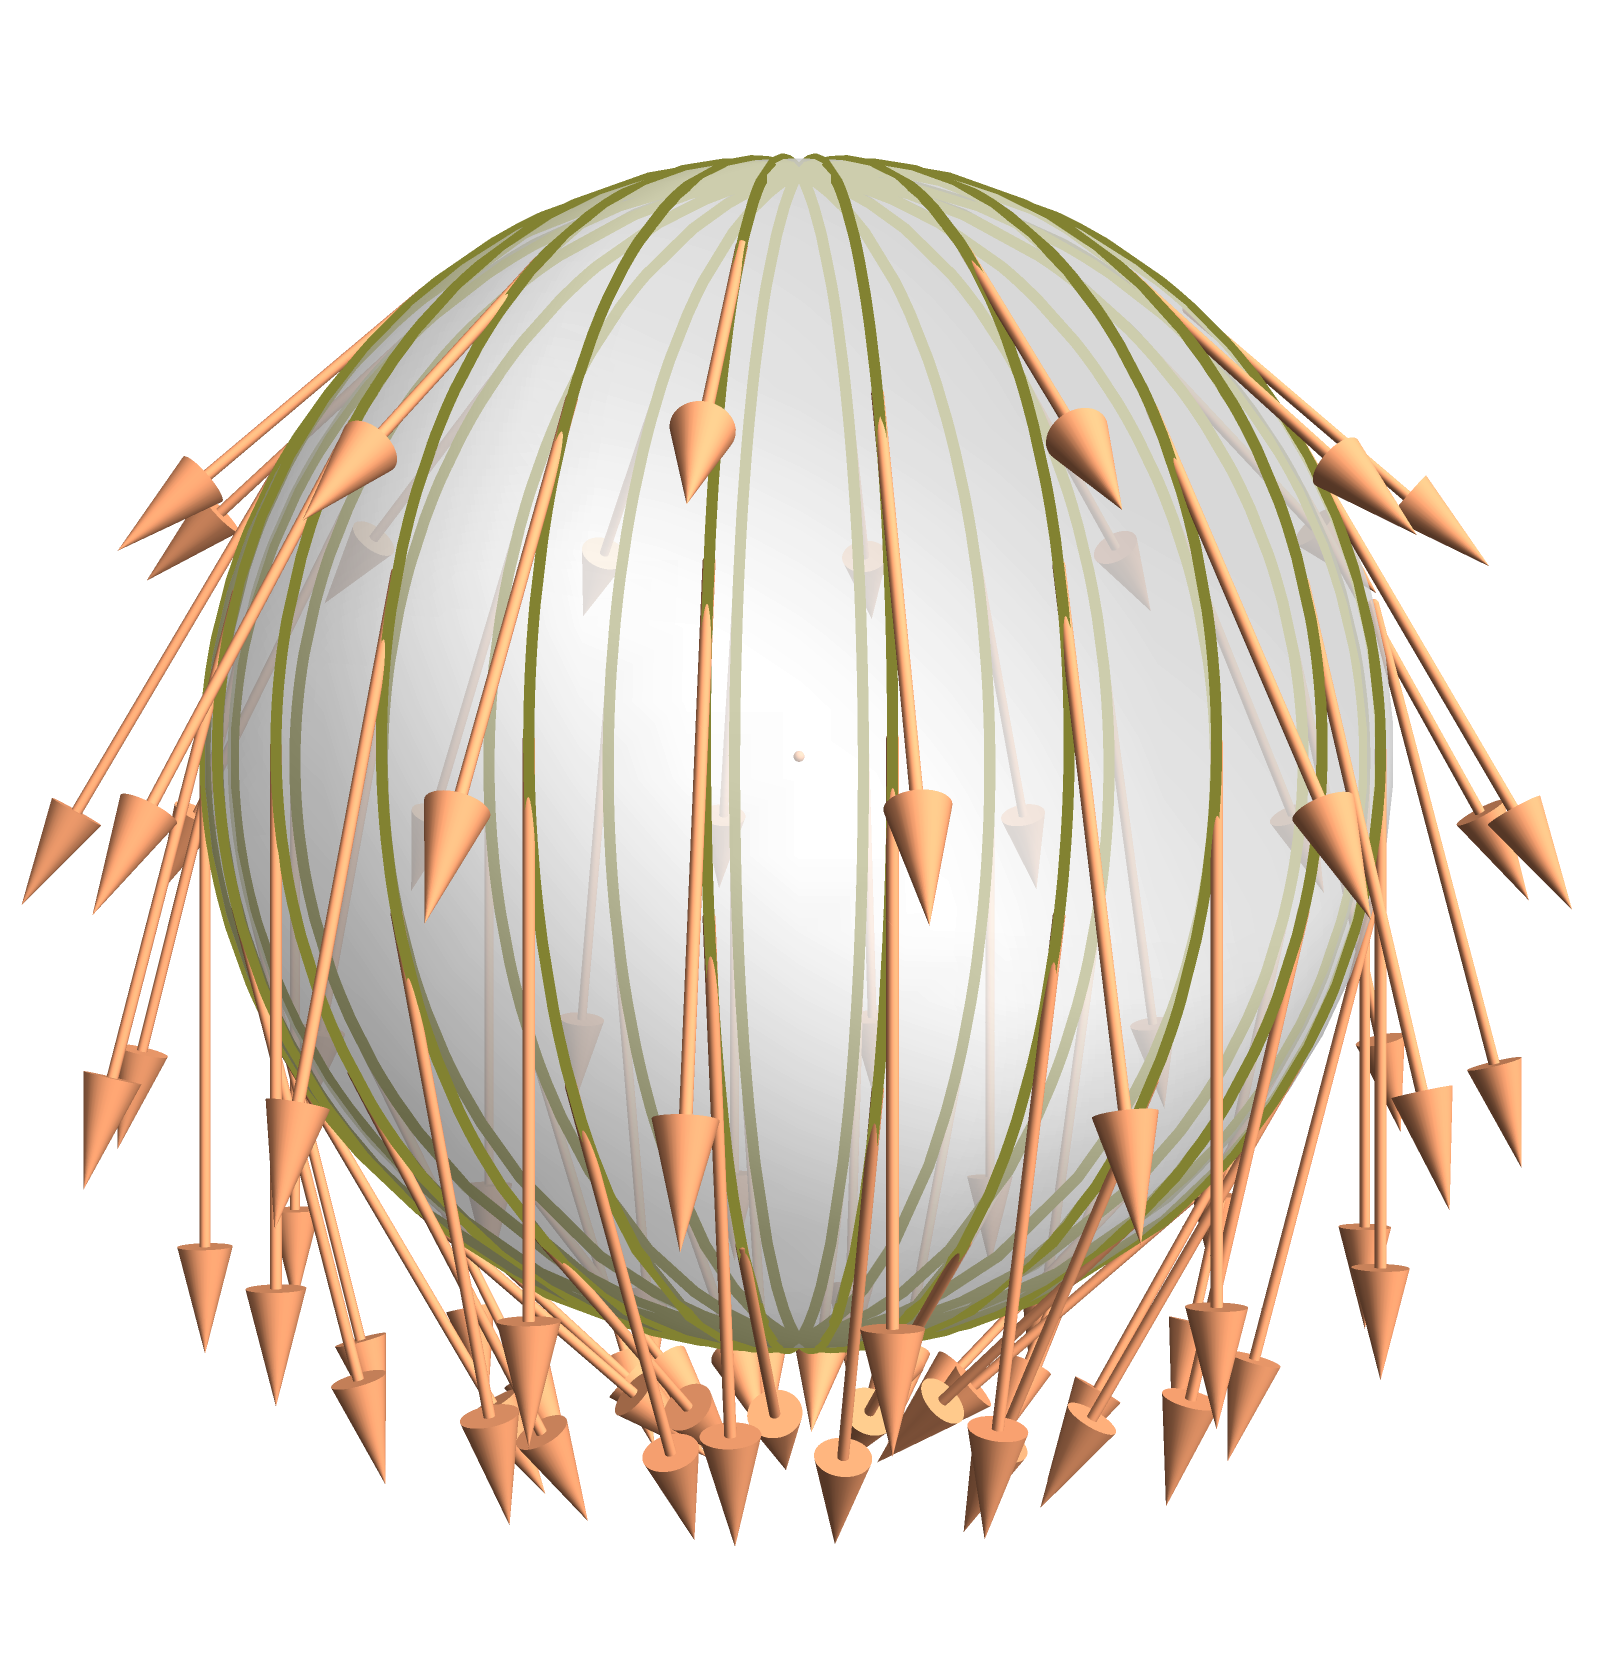
\includegraphics[height=2in]{conformalflow}
		\caption{The local flow of $X$.}
		\label{fig:conformalflow}
	\end{figure}
	
	This is an example of a \emph{complete vector field} since the local flow exists for all time at all points. If we had removed the Antarctic Circle from the sphere, this vector field would be incomplete (since the flow ceases to exist once you go over the edge).
\end{example}

With local flows in our toolkit we would then like to define the Lie derivative as something like
\[
	(\mathcal{L}_XY)(p) = \lim_{t \to 0} \frac{Y(\Phi_t(p)) - Y(p)}{t}.
\]
But if you think about it, the numerator in the difference quotient \emph{makes no sense!} After all, $Y(\Phi_t(p)) \in T_{\Phi_t(p)}M$ and $Y(p) \in T_pM$ live in completely different vector spaces. There's no sense in which we can subtract these two vectors.

So we need some way to get the tangent vectors determined by $Y$ at different points to be in the same tangent space.

Thus far, the only machines we have for moving tangent vectors between different tangent spaces are differentials of smooth maps. The only smooth map we have at our disposal is $\Phi_t$, so somehow that must come into play. One possibility is
\[
	\lim_{t \to 0} \frac{Y(\Phi_t(p)) - (d \Phi_t)_p Y(p)}{t}
\]
since both $Y(\Phi_t(p))$ and $(d \Phi_t)_pY(p)$ live in $T_{\Phi_t(p)}M$. The problem with this is that, as $t$ changes, $T_{\Phi_t(p)}M$ is also changing, so we're taking limits of vectors in different tangent spaces. Now, all these tangent vectors still live in $TM$, so this is in fact doable, but it would be better if all the vectors in the limit actually lived in the tangent space, ideally $T_pM$. 

We are finally ready to define the Lie derivative:

\begin{definition}\label{def:Lie derivative}
	Suppose $M$ is a manifold, $X,Y \in \mathfrak{X}(M)$, and $p \in M$. Then the \emph{Lie derivative} of $Y$ with respect to $X$ at $p$ is
	\[
		(\mathcal{L}_XY)(p) := \lim_{t \to 0} \frac{(d \Phi_{-t})_{\Phi_t(p)}Y(\Phi_t(p)) - Y(p)}{t},
	\]
	where $\Phi_t$ is the local flow for $X$.
\end{definition}

This is a lot of obnoxious notation, but let's try to unpack it. First of all, notice that $\Phi_{-t}(\Phi_t(p)) = p$, since we're just flowing forward in time by $t$ and then backwards for the same time. So
\[
	(d\Phi_{-t})_{\Phi_t(p)}\from T_{\Phi_t(p)}M \to T_p M.
\]
Hence, plugging in $Y(\Phi_t(p))$ gives $(d\Phi_{-t})_{\Phi_t(p)}Y(\Phi_t(p)) \in T_pM$, and the difference quotient and the limit make sense as happening entirely in $T_pM$. A (somewhat messy) picture is shown in \cref{fig:lie-derivative2}.

\begin{figure}[htbp]
	\centering
		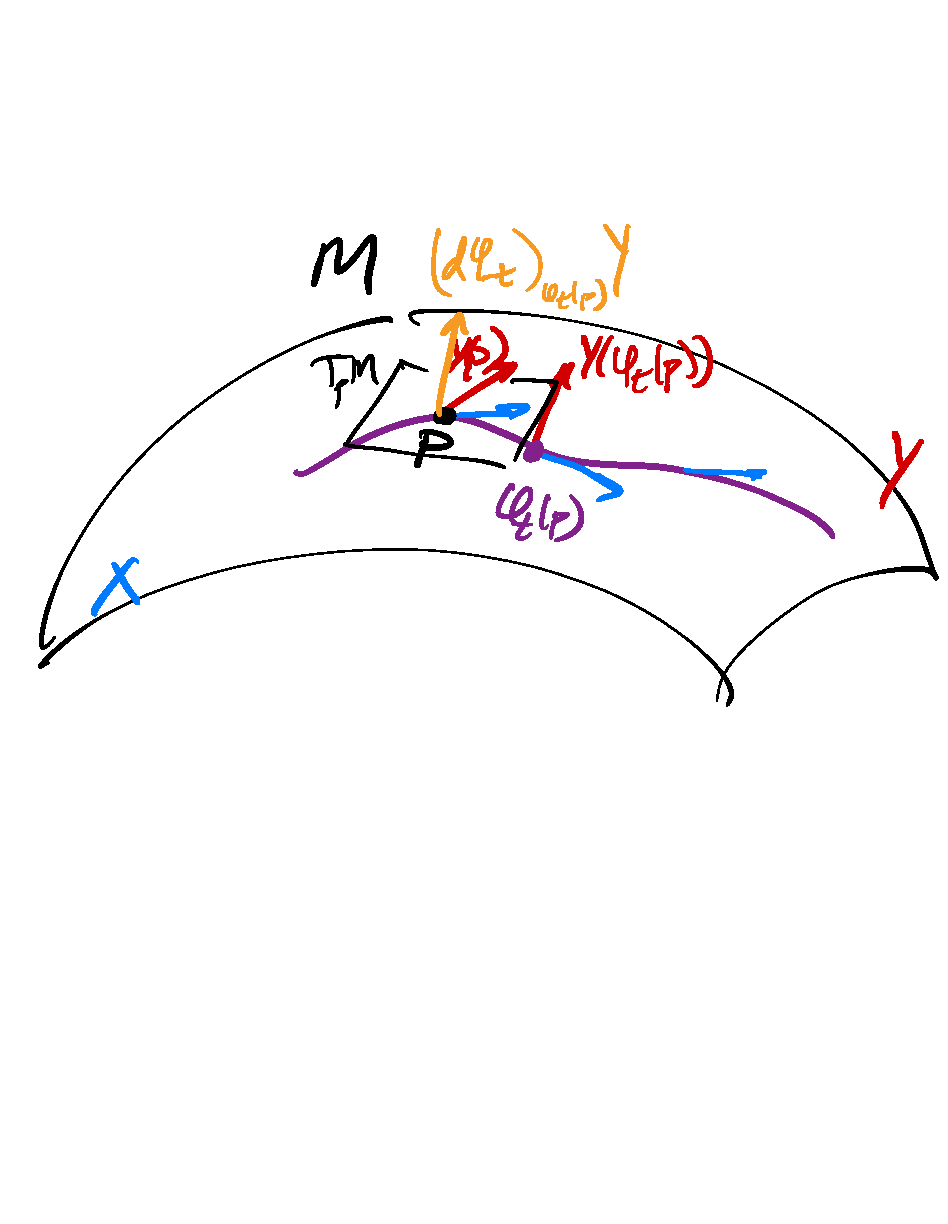
\includegraphics[height=1.5in]{lie-derivative-2}
	\caption{The pieces in the definition of $\mathcal{L}_XY$.}
	\label{fig:lie-derivative2}
\end{figure}

In looking at \cref{fig:lie-derivative2}, recall that the point was that we wanted to see how $Y$ varied as we moved in the direction of $X$. So at a point $p \in M$, we follow the local flow of $X$ for a small time $t$. $Y$ determines a tangent vector at the resulting point $\Phi_t(p)$. Now we push this vector $Y(\Phi_t(p))$ to $T_pM$ by the negative local flow of $X$ and compare to $Y(p)$.

You can imagine that if $Y$ had a constant magnitude and made a constant angle with $X$, then pushig $Y$ forward by the negative local flow (which is exactly $(d\Phi_{-t})_{\Phi_t(p)}Y(\Phi_t(p))$) would just give you the same vector you started with, namely $Y(p)$. But this makes sense: if $Y$ has a constant magnitude and makes a constant angle with $X$, then it's not changing at all with respect to $X$, and this derivative should really be 0.\footnote{You should take this paragraph figuratively and not literally: we don't have any notion of magnitude or angle for tangent vectors, because we don't yet have inner products on the tangent spaces. That will come when we start talking about Riemannian metrics!}

The slightly amazing fact is that the Lie derivative and the Lie bracket are the same:

\begin{proposition}\label{prop:Lie bracket = Lie derivative}
	Let $X,Y \in \mathfrak{X}(M)$ and choose $p \in M$. Then
	\[
		[X,Y](p) = (\mathcal{L}_XY)(p).
	\]
\end{proposition}

Notice, in particular, that this shows that the Lie derivative is antisymmetric:
\[
	\mathcal{L}_YX = [Y,X] = -[X,Y] = - \mathcal{L}_XY
\]
by the antisymmetry of the Lie bracket, which you might not have guessed from the definition of the Lie derivative.

\begin{proof}[Proof of \cref{prop:Lie bracket = Lie derivative}]
	Both expressions are tangent vectors at $p$, so formally they're differential operators evaluated on functions that are differentiable in a neighborhood of $p$. So we'll choose a test function $f$ which is differentiable in a neighborhood of $p$, and the goal is to show that
	\[
		\lim_{t \to 0} \frac{(d\Phi_{-t})_{\Phi_t(p)}Y(\Phi_t(p))-Y(p)}{t}(f)(p) = ((XY-YX)f)(p).
	\]
	Let's focus on the first term in the numerator, $\left((d\Phi_{-t})_{\Phi_t(p)}Y)f\right)(p)$:
	\[
		\left((d\Phi_{-t})_{\Phi_t(p)}Y)f\right)(p) = (df_p)(((d\Phi_{-t})_{\Phi_t(p)}Y)(p)) = (d(f \circ \Phi_{-t})_{\Phi_t(p)}Y(\Phi_t(p))) = (Y(f\circ \Phi_{-t}))(\Phi_t(p)),
	\]
	where we used \cref{lem:vector fields and differentials} for the first and last equalities\footnote{Note: I added this lemma after the initial draft, so it was not there when you previously read that section.} and the chain rule for the middle equality. Therefore,
	\[
		(\mathcal{L}_XY)(p) = \lim_{t \to 0} \frac{(Y(f \circ \Phi_{-t}))(\Phi_t(p))-(Yf)(p)}{t}.
	\]
	
	If we could turn this into something like 
	\begin{equation}\label{eq:XYf}
		\lim_{t \to 0} \frac{(Yf)(\Phi_t(p)) - (Yf)(p)}{t} = \left. \frac{d((Yf)\circ \Phi_t)}{dt} \right|_{t = 0} = (X(Yf))(p),
	\end{equation}
	we'd be in business.
	
	In fact, if we could write $f(\Phi_{-t}(q)) = f(q) + t g(t,q)$ for some function $g$, then we could get a term like~\eqref{eq:XYf} to appear because then we'd have
	\begin{align*}
		\lim_{t \to 0} \frac{(Y(f \circ \Phi_{-t}))(\Phi_t(p))-(Yf)(p)}{t} & = \lim_{t \to 0} \frac{(Y(f +t g(t, \cdot)))(\Phi_t(p))-(Yf)(p)}{t} \\
		& = \lim_{t \to 0} \frac{(Yf)(\Phi_t(p)) + (Y(t g(t, \cdot)))(\Phi_t(p))-(Yf)(p)}{t} \\
		& = \lim_{t \to 0} \frac{(Yf)(\Phi_t(p)) + t(Y( g(t, \cdot)))(\Phi_t(p))-(Yf)(p)}{t} \\
		& = \lim_{t \to 0} \frac{(Yf)(\Phi_t(p)) -(Yf)(p)}{t} + Y(g(0,\Phi_0(p)) \\
		& = (X(Yf))(p) + Y(g(0,p)).
	\end{align*}
	This will then equal $((XY-YX)f)(p)$ if we can find such a $g$ so that the expression $Y(g(0,p))$ is equal to $(Y(Xf))(p)$.
	
	But this is easy: rearranging $f(\Phi_{-t}(q)) = f(q) + tg(t,q)$ yields
	\[
		g(t,q) = \frac{f(\Phi_{-t}(q))-f(q)}{t},
	\]
	at least for $t \neq 0$. We can extend the definition to $t=0$ by taking the limit:
	\[
		g(0,q) := \lim_{t \to 0} \frac{f(\Phi_{-t}(q)) - f(q)}{t} = (Xf)(q),
	\]
	which is exactly what we need, since then $Y(g(0,p)) = (Y(Xf))(p)$.
\end{proof}

